% Presentación final INF659: la historia completa del trabajo con SAM sobre radar.
% Compilar con: pdflatex presentacion_final.tex (dos veces).
\documentclass[10pt,aspectratio=1610]{beamer}
\usetheme{Warsaw}
\usepackage[T1]{fontenc}
\usepackage[utf8]{inputenc}
\usepackage[spanish,es-noshorthands]{babel}
\usepackage{lmodern}
\usepackage{booktabs}
\usepackage{array}
\usepackage{pifont}
\usepackage{tikz}
\usetikzlibrary{arrows.meta,positioning,shapes.misc,calc}
\usepackage{pgfplots}
\pgfplotsset{compat=1.17, every axis/.append style={/pgf/number format/.cd, fixed, precision=3, 1000 sep={\,}}}
\graphicspath{{../../results/figuras/}{./}}

\setbeamertemplate{navigation symbols}{}

\newcommand{\si}{{\color{green!50!black}\ding{51}}}
\newcommand{\no}{{\color{red!70!black}\ding{55}}}
\newcommand{\fuente}[1]{\par\vfill{\tiny\color{gray}#1}}
\definecolor{samc}{HTML}{5B33A8}
\definecolor{unetc}{HTML}{0F8F87}
\definecolor{otsuc}{HTML}{9A9A9A}
\definecolor{umbc}{HTML}{C9A227}
\newcolumntype{L}[1]{>{\raggedright\arraybackslash}p{#1}}

\title[SAM sobre radar · la historia completa]{Segmentación de agua en imágenes de radar con SAM}
\subtitle{Qué probamos, qué funcionó y qué no}
\author[Arzapalo · Miranda · Zavala]{John Manuel Arzapalo Arana\\ Luis Alberto Miranda Mallqui\\ Juan Diego Zavala Viscardo}
\institute{INF659 · Técnicas Avanzadas de Data Mining y Sistemas Inteligentes\\ Pontificia Universidad Católica del Perú}
\date{Presentación final · noviembre de 2026}

\begin{document}

\begin{frame}
  \titlepage
\end{frame}

% =====================================================================
\section{Motivación}

\begin{frame}{Por qué importa: El Niño en el norte del Perú}
  \begin{columns}[T]
    \begin{column}{0.52\textwidth}
      \begin{tikzpicture}
        \begin{axis}[ybar, width=\linewidth, height=4.6cm, bar width=18pt,
            ymin=0, ymax=4200, ylabel={\scriptsize pérdidas (millones de US\$)},
            symbolic x coords={1982--83,1997--98,2017}, xtick=data,
            nodes near coords, every node near coord/.append style={font=\scriptsize},
            tick label style={font=\scriptsize}, axis lines*=left, ymajorgrids,
            grid style={gray!20}]
          \addplot[fill=red!55, draw=none] coordinates {(1982--83,3283) (1997--98,3500) (2017,3100)};
        \end{axis}
      \end{tikzpicture}
      {\tiny 11.6\,\%, 6.2\,\% y 1.6\,\% del PBI de cada época.}
    \end{column}
    \begin{column}{0.45\textwidth}
      \small
      \textbf{Niño Costero 2017}
      \begin{itemize}
        \item \textbf{162} fallecidos y 1.13 millones de afectados.
        \item \textbf{25\,700} viviendas colapsadas.
      \end{itemize}
      \textbf{2026--27}: ENFEN prevé un Niño costero de magnitud \textbf{extraordinaria}.
    \end{column}
  \end{columns}
  \begin{block}{La necesidad}
    En la emergencia el cielo está nublado: hay que saber \textbf{dónde está el agua} con radar, que ve a través de las nubes, y sin que una persona dibuje cada mapa.
  \end{block}
  \fuente{Fuentes: CAF/BCRP vía Andina (2023); OPS/OMS con SINPAD (2017); ENFEN, Comunicado Oficial N.º 19-2026.}
\end{frame}

\begin{frame}{La pregunta, los datos y cómo medimos}
  \begin{columns}[T]
    \begin{column}{0.5\textwidth}
      \textbf{Pregunta}
      \begin{itemize}\small
        \item ¿Sirve \textbf{SAM} (Meta, 2023), entrenado con 11 millones de fotos, para segmentar agua en \textbf{radar Sentinel-1}?
        \item Si no sirve tal cual, ¿qué hay que cambiar, y le gana a un modelo simple?
      \end{itemize}
      \textbf{Datos: Sen1Floods11}
      \begin{itemize}\small
        \item Recortes de 512$\times$512 px (10\,m), 11 inundaciones reales, máscaras dibujadas a mano.
        \item \textbf{train} 250 · \textbf{valid} 86 · \textbf{test} 89 · \textbf{Bolivia} 15 (región que ningún modelo vio).
      \end{itemize}
    \end{column}
    \begin{column}{0.47\textwidth}
      \textbf{Métrica}
      \[ \text{IoU} = \frac{TP}{TP+FP+FN} \]
      {\small \textbf{IoU global}: se suman los píxeles de todos los recortes. También se reporta el IoU medio por recorte.}

      \medskip
      \textbf{Evaluación}
      \begin{itemize}\small
        \item Todas las decisiones se toman con train y valid.
        \item \textbf{test} y \textbf{Bolivia} se evalúan \textbf{una sola vez}, al final.
        \item Intervalos de confianza del 95\,\% con bootstrap (5\,000 remuestreos).
      \end{itemize}
    \end{column}
  \end{columns}
\end{frame}

\begin{frame}{El recorrido en una línea de tiempo}
  \centering
  \resizebox{\linewidth}{!}{%
  \begin{tikzpicture}[
      hito/.style={circle, fill=blue!60!black, inner sep=2.2pt},
      caja/.style={draw=blue!40!black, fill=blue!5, rounded corners=2pt, align=left,
                   font=\scriptsize, text width=2.55cm, inner sep=3pt},
      tiempo/.style={fill=orange!85!black, text=white, rounded corners=2pt, font=\tiny\bfseries, inner sep=2pt}]
    \draw[-{Latex[length=3mm]}, line width=1.2pt, gray] (0,0) -- (11.4,0);
    \foreach \x/\f in {0.5/11-oct, 2.3/12-oct, 4.4/4-nov, 6.4/5-nov, 8.5/12-nov, 10.5/13-nov}{
      \node[hito] at (\x,0) {};
      \node[font=\scriptsize\bfseries, below=3pt] at (\x,0) {\f};
    }
    \node[caja, anchor=south] (a1) at (0.5,0.55) {\textbf{SAM tal como viene}\\ con puntos automáticos de Otsu};
    \node[caja, anchor=south] (a3) at (4.4,0.55) {\textbf{Adaptar SAM}\\ entrada en dB\\ LoRA en el codificador};
    \node[caja, anchor=south] (a5) at (8.5,0.55) {\textbf{Diagnóstico}\\ ¿por qué gana la U-Net?};
    \node[tiempo, above=1pt of a3] {74 min + 155 min};
    \node[tiempo, above=1pt of a5] {solo inferencia};
    \node[caja, anchor=north] (b2) at (2.3,-0.6) {\textbf{Disección de SAM}\\ y ajuste de solo el decodificador (4\,\%)};
    \node[caja, anchor=north] (b4) at (6.4,-0.6) {\textbf{U-Net, test y robustez}\\ evaluación final, 5 semillas, canal JRC};
    \node[caja, anchor=north] (b6) at (10.5,-0.6) {\textbf{Validación cruzada}\\ 10 regiones, una fuera cada vez};
    \node[tiempo, below=1pt of b2] {$\approx$2.5 min por entrenamiento};
    \node[tiempo, below=1pt of b4] {80 min + 5 min (test)};
    \node[tiempo, below=1pt of b6] {5.3 h de GPU};
  \end{tikzpicture}}

  \vspace{2mm}
  {\small Todo en una computadora con \textbf{RTX 3070 (8\,GB)}. Los cuatro bloques grandes suman $\approx$\textbf{10.5 h de GPU}.}
\end{frame}

% =====================================================================
\section{SAM tal cual}

\begin{frame}{Capítulo 1: SAM tal como viene}
  \begin{columns}[T]
    \begin{column}{0.55\textwidth}
      {\tiny\setlength{\tabcolsep}{0pt}%
      \begin{tabular*}{\linewidth}{@{\extracolsep{\fill}}cccc@{}}
        Radar (VH), Somalia & Otsu: IoU 0.18 & SAM original: IoU 0.20 & Etiqueta manual
      \end{tabular*}}\\[-1pt]
      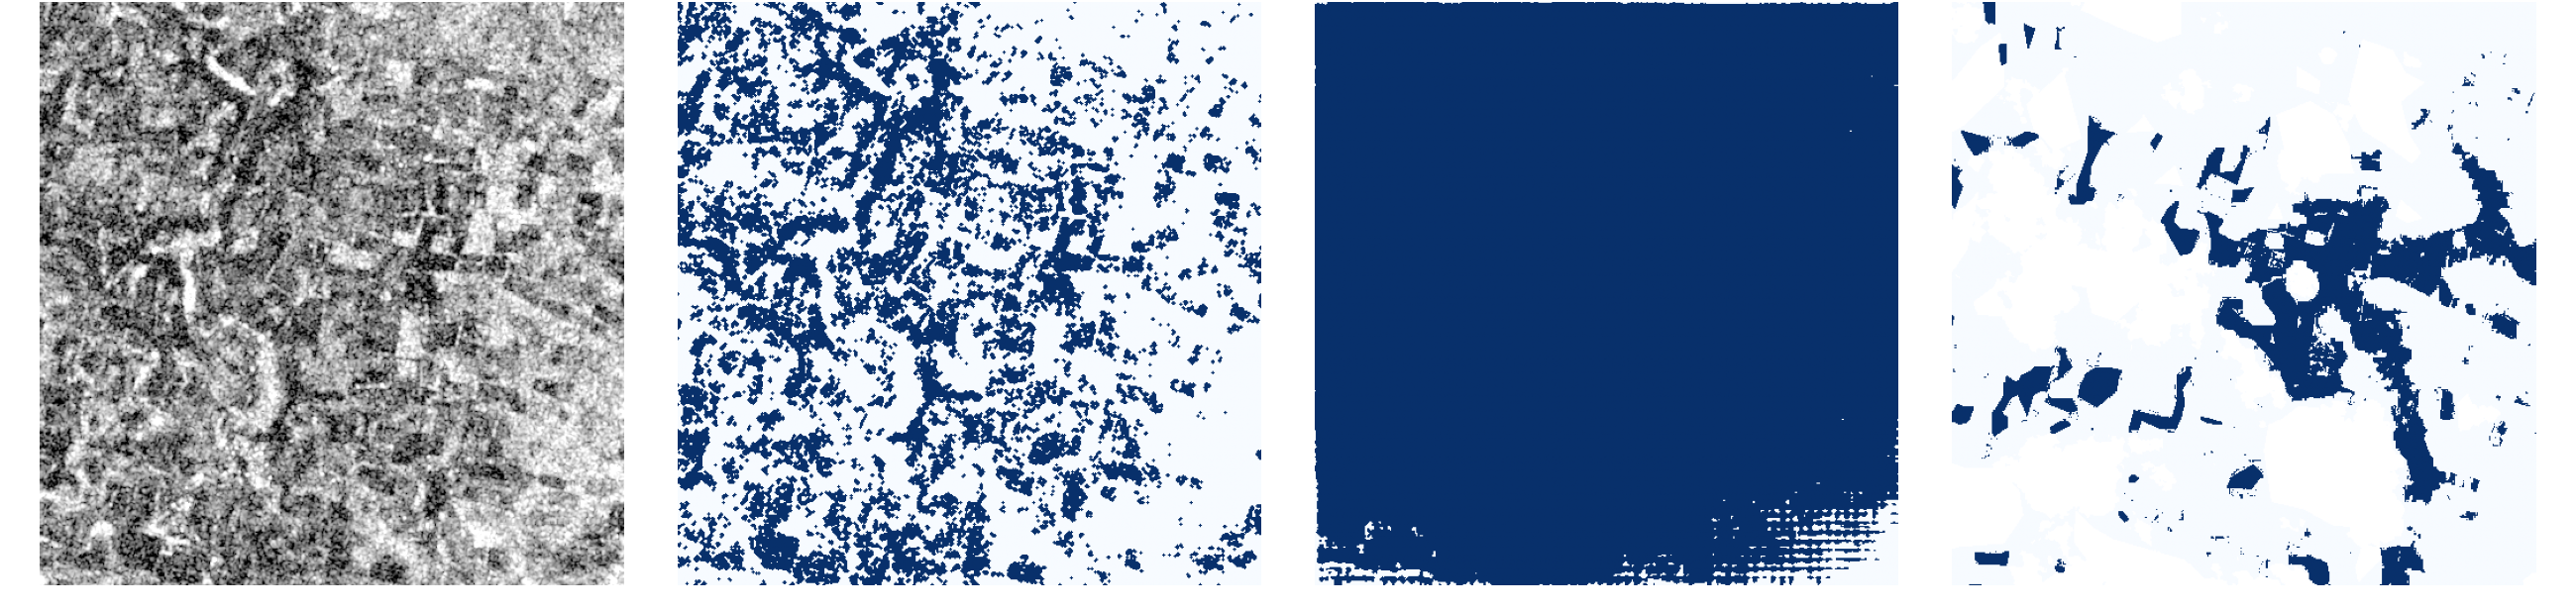
\includegraphics[width=\linewidth]{sam_original_somalia.png}

      \vspace{2mm}
      \begin{tikzpicture}
        \begin{axis}[ybar, width=\linewidth, height=3.6cm, bar width=20pt, ymin=0, ymax=0.32,
            symbolic x coords={Todo agua,Otsu,SAM}, xtick=data, nodes near coords,
            every node near coord/.append style={font=\scriptsize}, tick label style={font=\scriptsize},
            ylabel={\scriptsize IoU (86 recortes)}, axis lines*=left]
          \addplot[fill=otsuc, draw=none] coordinates {(Todo agua,0.11) (Otsu,0.256) (SAM,0.115)};
        \end{axis}
      \end{tikzpicture}
    \end{column}
    \begin{column}{0.43\textwidth}
      \small
      \begin{itemize}
        \item \textbf{Método}: Otsu separa oscuro (agua) de claro y de ahí salen 3 puntos positivos y 2 negativos para SAM. Sin intervención humana.
        \item SAM \textbf{pinta casi toda la imagen} de agua: rinde igual que decir «todo es agua».
        \item Otsu gana en 69 de 86 recortes.
      \end{itemize}
      \begin{alertblock}{Resultado}
        SAM no supera a Otsu: 0.115 contra 0.256 (IC 95\,\% de la diferencia $[-0.18,-0.10]$).
      \end{alertblock}
    \end{column}
  \end{columns}
\end{frame}

\begin{frame}{¿Qué pieza falla? El «ojo» o el «pincel»}
  \begin{columns}[T]
    \begin{column}{0.5\textwidth}
      \includegraphics[width=\linewidth]{valid_sonda_por_capa.png}
      {\scriptsize Sonda lineal por capa del codificador: AUC 0.934.}
    \end{column}
    \begin{column}{0.48\textwidth}
      \small
      \begin{tabular}{@{}L{0.72\linewidth}c@{}}
        \toprule
        Sospecha & ¿Es? \\ \midrule
        Los puntos: con puntos perfectos igual da 0.17 & \no \\
        El ojo (codificador): una recta separa agua y tierra (AUC 0.93) & \no \\
        La confianza de SAM: $\rho=-0.05$ con el acierto real & \si \\
        Elige la máscara más grande en 80 de 86 & \si \\
        \bottomrule
      \end{tabular}
    \end{column}
  \end{columns}
  \begin{block}{Conclusión}
    El codificador (96\,\% del modelo) \textbf{sí ve el agua}. Falla el decodificador: se autoevalúa mal y escoge la máscara equivocada.
  \end{block}
\end{frame}

\begin{frame}{Capítulo 2: reentrenar solo el decodificador (4\,\%)}
  \begin{columns}[c]
    \begin{column}{0.5\textwidth}
      \centering
      \begin{tikzpicture}[b/.style={draw, rounded corners, align=center, font=\scriptsize, minimum height=0.9cm}]
        \node[b, fill=gray!15, text width=2.4cm] (oj) {Codificador de imagen\\ 89.7\,M, \textbf{congelado}};
        \node[b, fill=gray!15, text width=2.4cm, below=0.35cm of oj] (pr) {Codificador de puntos\\ \textbf{congelado}};
        \coordinate (mid) at ($(oj.east)!0.5!(pr.east)$);
        \node[b, fill=green!15, draw=green!50!black, line width=1pt, text width=2.1cm, anchor=west] (de) at ($(mid)+(1.0,0)$) {Decodificador\\ 4.06\,M (\textbf{4\,\%})\\ \textbf{se entrena}};
        \draw[-Latex] (oj.east) -- (de); \draw[-Latex] (pr.east) -- (de);
      \end{tikzpicture}

      \vspace{2mm}
      \begin{itemize}\scriptsize
        \item Las salidas del codificador se \textbf{guardan una vez}: después cada experimento cuesta minutos.
        \item Una sola máscara de salida: ya no depende de la confianza rota.
        \item $\approx$\textbf{2.5 min por entrenamiento} en GPU, 3 semillas.
      \end{itemize}
    \end{column}
    \begin{column}{0.47\textwidth}
      \begin{tikzpicture}
        \begin{axis}[ybar, width=\linewidth, height=4.8cm, bar width=20pt, ymin=0, ymax=0.52,
            symbolic x coords={SAM original,Otsu,SAM + decodif.}, xtick=data, nodes near coords,
            every node near coord/.append style={font=\scriptsize}, tick label style={font=\scriptsize},
            ylabel={\scriptsize IoU valid}, axis lines*=left]
          \addplot[fill=samc!70, draw=none] coordinates {(SAM original,0.115) (Otsu,0.256) (SAM + decodif.,0.431)};
        \end{axis}
      \end{tikzpicture}
    \end{column}
  \end{columns}
  \begin{exampleblock}{Resultado}
    0.115 $\rightarrow$ \textbf{0.431 $\pm$ 0.038}: casi cuadruplica a SAM original y supera a Otsu en 57 de 86 recortes.
  \end{exampleblock}
\end{frame}

% =====================================================================
\section{Adaptar SAM}

\begin{frame}{Capítulo 3: cómo seguir mejorando a SAM}
  \small
  Revisamos trabajos parecidos y nuestro código, y encontramos tres cosas que cambiar:
  \vspace{2mm}
  \begin{center}\small
  \begin{tabular}{@{}lL{4.6cm}L{5.2cm}@{}}
    \toprule
    & Qué cambia & Por qué \\ \midrule
    1 & Entrada con rango fijo en dB, con VV y VH & la normalización por recorte borraba el nivel absoluto del radar, que es lo que distingue el agua \\[2pt]
    2 & LoRA en el codificador + rotaciones y espejados & el decodificador solo ya no daba más \\[2pt]
    3 & Una U-Net desde cero, con la misma entrada & ¿SAM aporta algo frente a una red simple? \\
    \bottomrule
  \end{tabular}
  \end{center}
\end{frame}

\begin{frame}{Entrada en dB: ayudó; elegir hiperparámetros en un subconjunto, no}
  \begin{columns}[c]
    \begin{column}{0.55\textwidth}
      \begin{tikzpicture}
        \begin{axis}[ybar, width=\linewidth, height=5.4cm, bar width=13pt, ymin=0, ymax=0.6,
            symbolic x coords={a,b,c}, xtick=data,
            xticklabels={{Como antes\\(por recorte)},{VH en dB\\(rango fijo)},{VV, VH y VV$-$VH\\en dB}},
            xticklabel style={align=center, font=\scriptsize}, tick label style={font=\scriptsize},
            nodes near coords, every node near coord/.append style={font=\tiny},
            ylabel={\scriptsize IoU valid (3 semillas)}, axis lines*=left, ymajorgrids, grid style={gray!20},
            area legend, legend style={font=\scriptsize, draw=none, fill=none, at={(0.5,1.03)}, anchor=south, legend columns=2, /tikz/every even column/.append style={column sep=8pt}},
            enlarge x limits=0.25]
          \addplot[fill=samc!75, draw=none] coordinates {(a,0.401) (b,0.472) (c,0.399)};
          \addplot[fill=samc!35, draw=none] coordinates {(a,0.418) (b,0.421) (c,0.439)};
          \legend{con puntos de Otsu, sin puntos}
          \draw[dashed, gray] (axis cs:a,0.431) -- (axis cs:c,0.431);
        \end{axis}
      \end{tikzpicture}
      {\tiny Línea punteada: SAM + decodificador con la entrada anterior (0.431).}
    \end{column}
    \begin{column}{0.43\textwidth}
      \scriptsize
      \begin{itemize}
        \item Solo se entrena el decodificador; el codificador sigue congelado. 74 min en total.
        \item \si\ \textbf{VH en dB con rango fijo}: +0.071 con el mismo entrenamiento. Mejor resultado: \textbf{0.472 $\pm$ 0.017}.
        \item \no\ \textbf{Agregar VV y VV$-$VH}: $-0.073$ y muy inestable. Un codificador entrenado con fotos no entiende polarizaciones.
        \item \no\ \textbf{Elegir lr y época en un subconjunto de train} (51 recortes, 60 candidatos) sobrestimó valid entre 0.06 y 0.22: quedarse con el máximo de muchos candidatos engaña.
      \end{itemize}
    \end{column}
  \end{columns}
\end{frame}

\begin{frame}{LoRA: adaptar el codificador de SAM}
  \begin{columns}[c]
    \begin{column}{0.55\textwidth}
      \begin{tikzpicture}
        \begin{axis}[ybar, width=\linewidth, height=5.4cm, bar width=14pt, ymin=0.4, ymax=0.66,
            symbolic x coords={a,b,c}, xtick=data,
            xticklabels={{VH en dB\\con puntos},{VV, VH, VV$-$VH\\con puntos},{VH en dB\\sin puntos}},
            xticklabel style={align=center, font=\scriptsize}, tick label style={font=\scriptsize},
            nodes near coords, every node near coord/.append style={font=\tiny},
            ylabel={\scriptsize IoU valid}, axis lines*=left, ymajorgrids, grid style={gray!20},
            area legend, legend style={font=\scriptsize, draw=none, fill=none, at={(0.5,1.03)}, anchor=south, legend columns=2, /tikz/every even column/.append style={column sep=8pt}},
            enlarge x limits=0.25]
          \addplot[fill=samc!75, draw=none] coordinates {(a,0.596) (b,0.601) (c,0.602)};
          \addplot[fill=samc!35, draw=none] coordinates {(a,0.591) (b,0.615) (c,0.596)};
          \legend{un modelo (media de 3), ensamble de 3 + TTA}
          \draw[dashed, gray] (axis cs:a,0.472) -- (axis cs:c,0.472);
        \end{axis}
      \end{tikzpicture}
      {\tiny Línea punteada: solo el decodificador con entrada en dB (0.472).}
    \end{column}
    \begin{column}{0.43\textwidth}
      \scriptsize
      \begin{itemize}
        \item LoRA de rango 8 en las 12 capas de atención, más el decodificador: \textbf{4.35\,M parámetros entrenables} (4.6\,\% de SAM).
        \item 9 entrenamientos de 15.6 min: 155 min en total. LoRA cupo en 4.3\,GB de la GPU.
        \item \si\ Sube unos \textbf{+0.12} sobre el mejor resultado con el codificador congelado.
        \item \si\ Ahora VV y VV$-$VH sí ayudan: el codificador aprende a usarlos.
        \item El modelo elegido para test: \textbf{SAM + LoRA con VV, VH y VV$-$VH}, ensamble de 3 semillas + TTA (0.615).
      \end{itemize}
    \end{column}
  \end{columns}
\end{frame}

\begin{frame}{La sorpresa: una U-Net simple gana en valid}
  \centering\small
  \begin{tabular}{@{}lcc@{}}
    \toprule
    & SAM + LoRA & U-Net desde cero \\ \midrule
    Preentrenamiento & 11 M de fotos & ninguno \\
    Parámetros totales & 93.7\,M & 7.76\,M \\
    Parámetros entrenados & 4.35\,M & 7.76\,M \\
    Tiempo por semilla & 15 min & 10 min \\
    \textbf{IoU valid} (media de 3) & 0.601 $\pm$ 0.010 & \textbf{0.637 $\pm$ 0.003} \\
    Ensamble + TTA & 0.615 & \textbf{0.642} \\
    \bottomrule
  \end{tabular}

  \vspace{3mm}
  \begin{columns}[T]
    \begin{column}{0.48\textwidth}
      \small
      \begin{itemize}
        \item La U-Net gana en las 3 semillas (+0.027 a +0.042) y varía 3 veces menos.
      \end{itemize}
    \end{column}
    \begin{column}{0.48\textwidth}
      \small
      \begin{itemize}
        \item \no\ \textbf{Pérdida Tversky} en SAM (castigar más el agua perdida): 0.615, mejora no significativa.
      \end{itemize}
    \end{column}
  \end{columns}
  \begin{alertblock}{Lo que cambia la historia}
    La entrada bien normalizada y las rotaciones bastan para que una red pequeña aprenda con solo 250 recortes.
  \end{alertblock}
\end{frame}

\begin{frame}{Cómo subió el IoU en valid}
  \centering
  \begin{tikzpicture}
    \begin{axis}[ybar, width=\linewidth, height=6.4cm, bar width=24pt, ymin=0, ymax=0.75,
        symbolic x coords={a,b,c,d,e,f,g},
        xtick={a,b,c,d,e,f,g},
        xticklabels={{SAM\\original},{Otsu},{SAM +\\decodificador},{SAM +\\decodificador\\entrada en dB},{SAM +\\LoRA},{SAM + LoRA\\ensamble + TTA},{U-Net\\desde cero}},
        xticklabel style={align=center, font=\scriptsize}, nodes near coords,
        every node near coord/.append style={font=\scriptsize},
        tick label style={font=\scriptsize}, ylabel={\scriptsize IoU global, valid (86 recortes)},
        axis lines*=left, ymajorgrids, grid style={gray!20}, enlarge x limits=0.08]
      \addplot[fill=samc!75, draw=none, bar shift=0pt] coordinates {(a,0.115) (c,0.431) (d,0.472) (e,0.601) (f,0.615)};
      \addplot[fill=otsuc, draw=none, bar shift=0pt] coordinates {(b,0.256)};
      \addplot[fill=unetc, draw=none, bar shift=0pt] coordinates {(g,0.637)};
    \end{axis}
  \end{tikzpicture}

  {\scriptsize Morado: SAM · gris: método clásico · verde azulado: U-Net. Las barras de SAM con más de una semilla muestran la media de 3.}
\end{frame}

% =====================================================================
\section{Test y generalización}

\begin{frame}{Capítulo 4: test y Bolivia, evaluados una sola vez}
  \centering
  \begin{tikzpicture}
    \begin{axis}[ybar, width=0.95\linewidth, height=5.2cm, bar width=17pt, ymin=0, ymax=0.78,
        symbolic x coords={Otsu,Umbral fijo filtrado,SAM + LoRA,U-Net}, xtick=data,
        nodes near coords, every node near coord/.append style={font=\tiny},
        tick label style={font=\scriptsize}, ylabel={\scriptsize IoU global},
        axis lines*=left, ymajorgrids, grid style={gray!20}, enlarge x limits=0.15,
        area legend, legend style={font=\scriptsize, draw=none, fill=none, at={(0.5,1.03)}, anchor=south, legend columns=2, /tikz/every even column/.append style={column sep=8pt}}]
      \addplot[fill=blue!55!black, draw=none] coordinates {(Otsu,0.263) (Umbral fijo filtrado,0.582) (SAM + LoRA,0.642) (U-Net,0.666)};
      \addplot[fill=orange!80!black, draw=none] coordinates {(Otsu,0.467) (Umbral fijo filtrado,0.613) (SAM + LoRA,0.657) (U-Net,0.628)};
      \legend{{test (89 recortes de regiones conocidas)}, {Bolivia (15 recortes, región no vista)}}
    \end{axis}
  \end{tikzpicture}
  \begin{columns}[T]
    \begin{column}{0.5\textwidth}
      \scriptsize
      \begin{itemize}
        \item Los modelos se fijaron antes de abrir test. Otsu y el umbral fijo son las referencias clásicas.
        \item SAM + LoRA: \textbf{0.642} en test y \textbf{0.657} en Bolivia, frente a 0.263 y 0.467 de Otsu.
      \end{itemize}
    \end{column}
    \begin{column}{0.48\textwidth}
      \scriptsize
      \begin{itemize}
        \item En test gana la U-Net (0.666). \textbf{En Bolivia, la región que nadie vio, gana SAM.}
        \item Con la métrica del paper del dataset (IoU medio por recorte), superamos su modelo con etiquetas manuales.
      \end{itemize}
    \end{column}
  \end{columns}
\end{frame}

\begin{frame}{Bolivia: cómo se ven las predicciones}
  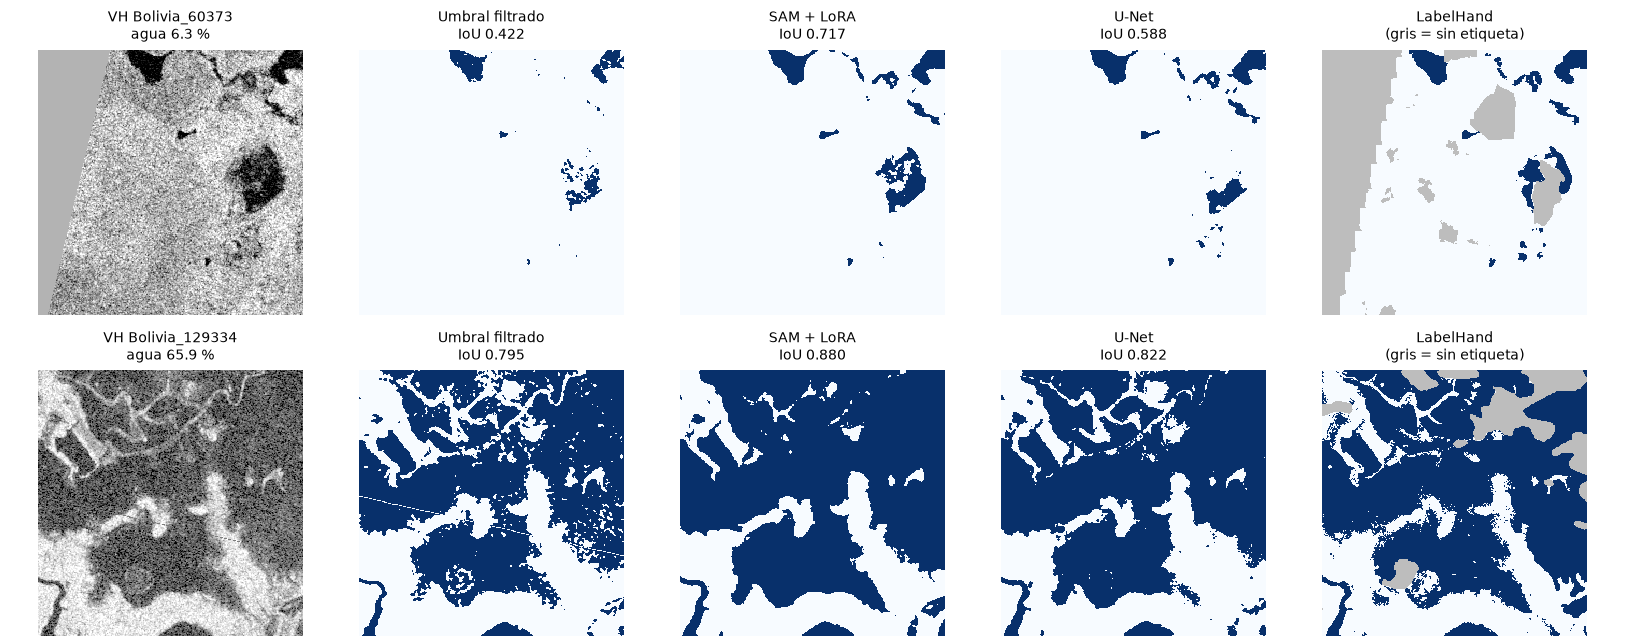
\includegraphics[width=\linewidth]{bolivia_ejemplos.png}
  \small
  \begin{itemize}
    \item Arriba: SAM recupera mejor la laguna de la derecha (0.72 contra 0.59 de la U-Net).
    \item Abajo, con 66\,\% de agua: los tres métodos aciertan lo grueso; el umbral deja ruido.
    \item Gris en la etiqueta: zonas sin etiquetar, que no cuentan.
  \end{itemize}
\end{frame}

\begin{frame}{Robustez: ¿se sostiene lo que vimos?}
  \small
  \begin{columns}[T]
    \begin{column}{0.5\textwidth}
      \textbf{Una línea base clásica fuerte}
      \begin{itemize}\scriptsize
        \item Umbral fijo en VH ($-23.3$\,dB) con filtro de mediana, elegido solo en train.
        \item Test 0.582, Bolivia 0.613: \textbf{mucho mejor que Otsu}.
        \item En Bolivia la ventaja de los modelos sobre él ya no es concluyente.
      \end{itemize}
      \textbf{Cinco semillas}
      \begin{itemize}\scriptsize
        \item SAM 0.603 $\pm$ \textbf{0.017}; U-Net 0.635 $\pm$ \textbf{0.004}.
        \item SAM varía 4 veces más: por eso el ensamble le importa tanto.
      \end{itemize}
    \end{column}
    \begin{column}{0.48\textwidth}
      \textbf{IoU global contra IoU medio}
      \begin{itemize}\scriptsize
        \item Test: 0.642 global, 0.405 medio.
        \item Un tercio de los recortes tiene $<$1\,\% de agua: pesan 3\,\% de los píxeles, pero un error pequeño los deja con IoU $\approx 0$.
        \item Mapeamos bien el área inundada; fallamos más en imágenes casi secas.
      \end{itemize}
      \textbf{Agua permanente (JRC) como canal extra}
      \begin{itemize}\scriptsize
        \item Valid +0.010, pero \textbf{Bolivia $-0.111$}: el modelo deja de marcar agua donde el mapa no la tenía.
      \end{itemize}
    \end{column}
  \end{columns}
\end{frame}

\begin{frame}{Lo que no funcionó (y lo que nos enseñó)}
  \small
  \renewcommand{\arraystretch}{1.15}
  \begin{tabular}{@{}L{0.35\linewidth}L{0.18\linewidth}L{0.40\linewidth}@{}}
    \toprule
    Intento & Resultado & Lección \\ \midrule
    SAM con puntos automáticos & 0.115 & la confianza de SAM no sirve en radar \\
    Más puntos o puntos perfectos & $\le$ 0.17 & el problema no eran los puntos \\
    VV + VH con el codificador congelado & $-0.073$ & los canales nuevos piden adaptar el codificador \\
    Elegir época y lr en un subconjunto de train & sobrestima 0.06--0.22 & con pocos datos, quedarse con el máximo engaña \\
    Pérdida Tversky & +0.014, no significativo & mover el equilibrio entre errores no basta \\
    Canal de agua permanente (JRC) & Bolivia $-0.111$ & una pista fácil daña la generalización \\
    Promediar SAM y U-Net & +0.001 & los dos fallan en los mismos píxeles \\
    \bottomrule
  \end{tabular}
\end{frame}

\begin{frame}{Capítulo 5: ¿por qué pierde SAM si tiene 12 veces más parámetros?}
  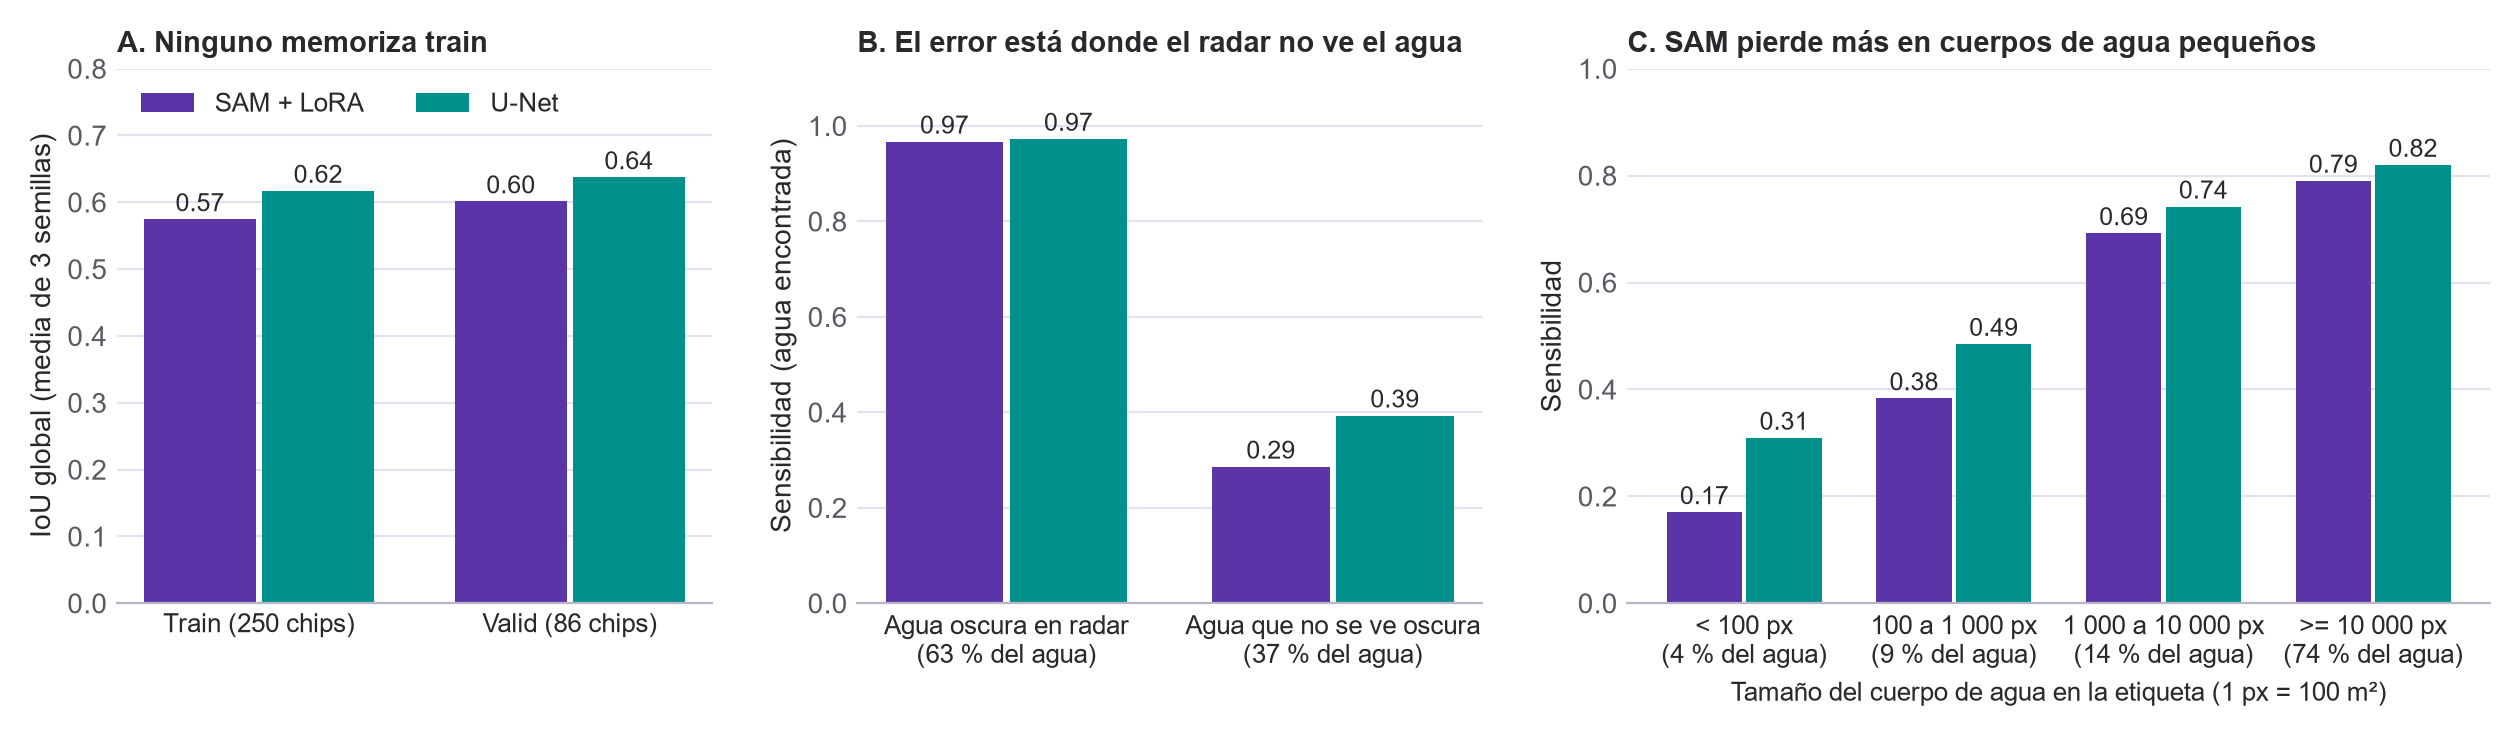
\includegraphics[width=\linewidth]{diagnostico_sam_vs_unet.png}
  \begin{columns}[T]
    \begin{column}{0.5\textwidth}
      \scriptsize
      \begin{itemize}
        \item \textbf{Nadie memoriza}: a SAM le falta ajuste, no le sobra.
        \item SAM entrena \textbf{menos} parámetros (4.35\,M contra 7.76\,M); el resto está congelado y aprendió con fotos.
      \end{itemize}
    \end{column}
    \begin{column}{0.48\textwidth}
      \scriptsize
      \begin{itemize}
        \item El límite lo pone \textbf{el radar}: los dos hallan el 97\,\% del agua oscura y fallan en el 37\,\% que no se ve oscura.
        \item SAM pierde más detalle fino: halla la mitad de los cuerpos de agua pequeños.
      \end{itemize}
    \end{column}
  \end{columns}
  \fuente{La literatura coincide: en Sen1Floods11 una U-Net desde cero queda primera dentro de las regiones de entrenamiento (PANGAEA 2024; Marti-Escofet et al. 2025).}
\end{frame}

\begin{frame}{Capítulo 6: validación cruzada dejando una región fuera}
  \begin{columns}[c]
    \begin{column}{0.55\textwidth}
      \centering
      \begin{tikzpicture}[r/.style={minimum width=0.42cm, minimum height=0.36cm, draw=white, line width=0.6pt}]
        \foreach \reg [count=\i from 0] in {Ghana,India,Mekong,Nigeria,Pakistan,Paraguay,Somalia,Spain,Sri-Lanka,USA}{
          \foreach \j in {0,...,9}{
            \ifnum\i=\j
              \node[r, fill=orange!80!black] at (\j*0.44, -\i*0.38) {};
            \else
              \node[r, fill=blue!35] at (\j*0.44, -\i*0.38) {};
            \fi
          }
          \node[font=\tiny, anchor=east] at (-0.3, -\i*0.38) {\reg\ fuera};
          \node[font=\tiny, anchor=south west, rotate=50] at (\i*0.44-0.12, 0.25) {\reg};
        }
      \end{tikzpicture}

      {\scriptsize Cada fila es un pliegue. Azul: regiones con las que se entrena · naranja: la región que se predice sin haberla visto.}
    \end{column}
    \begin{column}{0.43\textwidth}
      \small
      \begin{itemize}
        \item \textbf{Pregunta}: ¿SAM generaliza mejor que la U-Net a regiones nuevas? Bolivia lo insinuaba, pero con 15 recortes.
        \item train + valid: \textbf{336 recortes}. Test y Bolivia no se tocan.
        \item Mismas recetas, semilla 0, sin búsqueda de hiperparámetros.
        \item Se declara un ganador solo si el IC 95\,\% por región excluye el cero.
        \item 10 pliegues de 28--46 min: \textbf{5.3 h de GPU}.
      \end{itemize}
    \end{column}
  \end{columns}
\end{frame}

\begin{frame}{Resultado: en regiones nuevas, empate}
  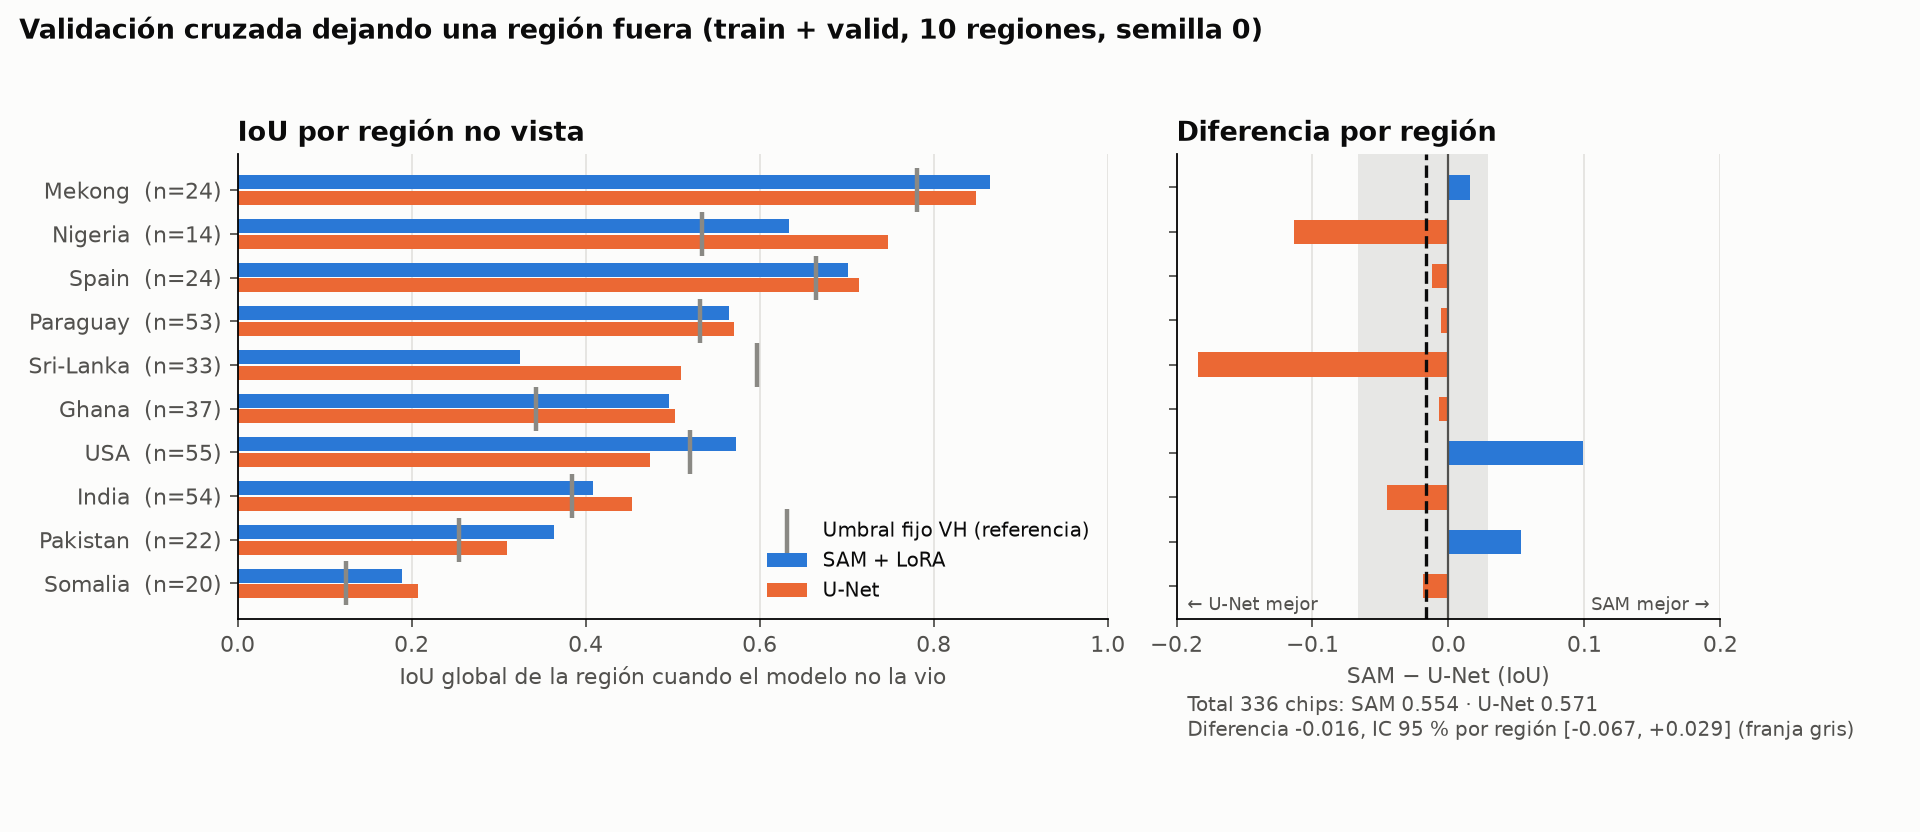
\includegraphics[width=\linewidth]{validacion_por_region.png}
  \begin{columns}[T]
    \begin{column}{0.5\textwidth}
      \scriptsize
      \begin{itemize}
        \item SAM 0.554, U-Net 0.571: $-0.017$, IC $[-0.067, +0.029]$. \textbf{No hay diferencia significativa.}
        \item La U-Net gana en 7 regiones y SAM en 3.
      \end{itemize}
    \end{column}
    \begin{column}{0.48\textwidth}
      \scriptsize
      \begin{itemize}
        \item \textbf{La región pesa más que el modelo}: de 0.19 (Somalia) a 0.86 (Mekong).
        \item Los dos superan al umbral fijo en 8 o 9 de las 10 regiones.
      \end{itemize}
    \end{column}
  \end{columns}
\end{frame}

\begin{frame}{Dónde sí destaca SAM: fuera de las regiones de entrenamiento}
  \begin{columns}[T]
    \begin{column}{0.5\textwidth}
      \begin{tikzpicture}
        \begin{axis}[ybar, width=\linewidth, height=4.8cm, bar width=16pt, ymin=0.5, ymax=0.68,
            symbolic x coords={vista,novista}, xtick=data,
            xticklabels={{región vista\\al entrenar},{región no vista\\(validación cruzada)}},
            xticklabel style={align=center, font=\scriptsize}, tick label style={font=\scriptsize},
            nodes near coords, every node near coord/.append style={font=\scriptsize},
            ylabel={\scriptsize IoU, mismos 86 recortes de valid}, axis lines*=left, ymajorgrids, grid style={gray!20},
            area legend, legend style={font=\scriptsize, draw=none, fill=none, at={(0.5,1.03)}, anchor=south, legend columns=2, /tikz/every even column/.append style={column sep=8pt}},
            enlarge x limits=0.45]
          \addplot[fill=samc!80, draw=none] coordinates {(vista,0.612) (novista,0.587)};
          \addplot[fill=unetc, draw=none] coordinates {(vista,0.639) (novista,0.584)};
          \legend{SAM + LoRA, U-Net}
        \end{axis}
      \end{tikzpicture}
      {\scriptsize SAM cae 0.025; la U-Net, 0.055.}
    \end{column}
    \begin{column}{0.48\textwidth}
      \small
      \begin{itemize}
        \item \textbf{Bolivia}: SAM 0.657 contra 0.628, y gana en 10 de los 15 recortes.
        \item \textbf{Se degrada menos al cambiar de región}: la ventaja de la U-Net desaparece cuando la región es nueva (0.587 contra 0.584).
        \item \textbf{Menos falsas alarmas}: en las 10 regiones, precisión de 0.76 contra 0.71 de la U-Net, con 32\,\% menos píxeles marcados como agua sin serlo.
        \item Gana con claridad en \textbf{USA} (+0.098) y \textbf{Pakistan} (+0.053).
      \end{itemize}
    \end{column}
  \end{columns}
  \vspace{1mm}
  \begin{block}{Lectura}
    \small El preentrenamiento de SAM le da \textbf{más estabilidad ante regiones no vistas} y un mapa más conservador. A cambio deja más agua sin marcar (sensibilidad 0.67 contra 0.75), y con 10 regiones la diferencia total no es significativa.
  \end{block}
\end{frame}

% =====================================================================
\section{Cierre}

\begin{frame}{Cuánto costó cada etapa}
  \centering\small
  \begin{tabular}{@{}lrl@{}}
    \toprule
    Etapa & Tiempo & Qué se entrenó \\ \midrule
    SAM tal como viene, con puntos de Otsu & minutos & nada \\
    Disección de SAM y ajuste del decodificador & $\approx$2.5 min por modelo & decodificador, 3 semillas \\
    Entrada en dB (solo decodificador) & 74 min & 6 configuraciones y 3 lr \\
    LoRA en el codificador & 155 min & 9 modelos de 15.6 min \\
    U-Net y pérdida Tversky & 80 min & 6 modelos \\
    Evaluación en test y Bolivia & 5 min & nada \\
    Cinco semillas y canal JRC & --- & 7 modelos \\
    Diagnóstico SAM contra U-Net & minutos & nada \\
    Validación cruzada por región & 5.3 h & 20 modelos \\
    \bottomrule
  \end{tabular}

  \vspace{4mm}
  \begin{block}{Lo que lo hizo posible en una sola computadora}
    \small Guardar la salida del codificador de SAM (cada prueba del decodificador pasó de horas a minutos) y ahorrar memoria en el entrenamiento: SAM con LoRA cupo en 4.3\,GB de una RTX 3070.
  \end{block}
\end{frame}

\begin{frame}{Conclusiones}
  \begin{enumerate}
    \item \textbf{SAM tal como viene no sirve en radar}: no por los puntos ni por el codificador, sino porque su decodificador elige mal la máscara.
    \item \textbf{Reentrenar solo el 4\,\% lo cuadruplica} (0.115 $\rightarrow$ 0.431). Con la entrada en dB y LoRA llega a \textbf{0.642 en test} y \textbf{0.657 en Bolivia}.
    \item \textbf{Una U-Net desde cero lo iguala o lo supera} dentro de las regiones de entrenamiento (0.666 en test). Más parámetros preentrenados no bastan.
    \item \textbf{Fuera de esas regiones SAM se sostiene mejor}: gana en Bolivia, pierde menos al cambiar de región y da menos falsas alarmas. En 10 regiones nuevas, los dos empatan.
    \item \textbf{El techo lo pone el sensor}: el agua que el radar no muestra oscura es casi todo el error de ambos modelos.
  \end{enumerate}
\end{frame}

\begin{frame}
  \centering
  \vfill
  {\Huge\color{blue!60!black}\textbf{¡Gracias!}}\par
  \vspace{4mm}
  {\Large ¿Preguntas?}\par
  \vfill
  {\scriptsize Bonafilia et al. (2020) · Kirillov et al. (2023) · Hu et al. (2022, LoRA) · Ronneberger et al. (2015, U-Net) · Otsu (1979) · Garg et al. (2023) · Marsocci et al. (2024, PANGAEA) · Marti-Escofet et al. (2025) · ENFEN (2026) · OPS/OMS (2017)}
  \vfill
\end{frame}

\end{document}
